\documentclass[12pt, fleqn]{article}
\usepackage[portuguese]{babel}
\usepackage{newpxtext, newpxmath}
\usepackage{amsmath}
\usepackage{titling}
\usepackage{enumitem}
\usepackage{geometry}
\usepackage{graphicx}
\usepackage{float}
\usepackage{listings}
\usepackage{xcolor}

\graphicspath{{./images/}}

\geometry{
    paper=a4paper,
    top=64pt,
    bottom=64pt,
    left=112pt,
    right=112pt
}

\lstset{
    basicstyle=\ttfamily\small,
    backgroundcolor=\color{gray!5},
    frame=single,
    rulecolor=\color{gray!20},
    framesep=16pt,
    xleftmargin=16pt,
    xrightmargin=16pt,
    captionpos=b
}

\renewcommand{\arraystretch}{1.2}

\setlength{\tabcolsep}{8pt}

\NewDocumentCommand{\course}{m}{\gdef\thecourse{#1}}
\NewDocumentCommand{\authors}{m}{\gdef\theauthors{#1}}
\NewDocumentCommand{\professor}{m}{\gdef\theprofessor{#1}}
\NewDocumentCommand{\semester}{m}{\gdef\thesemester{#1}}

\renewcommand{\maketitle}{
    \begin{titlepage}
        \begin{center}
            {\scshape Universidade Federal do Rio Grande do Sul\\Instituto de Informática} \\
            \vspace*{\fill}
            {\large \thecourse} \\[16pt]
            {\Huge \thetitle} \\[36pt]
            \theauthors \\
            \vspace*{\fill}
            \theprofessor \\[2pt]
            \thesemester
        \end{center}
    \end{titlepage}
}

\course{Circuitos Digitais – INF01058}
\title{LAB 07 – Divisor de frequência}
\authors{
    Ana Cláudia Rodrigues — 343123 \\[2pt]
    Bruno Samuel Ardenghi Gonçalves — 550452
}
\professor{Prof. Mateus Grellert}
\semester{2025/1}

\begin{document}

\maketitle

\section{Introdução}

Neste laboratório desenvolvemos um divisor de frequência usando circuitos sequenciais, com o intuito de, a partir de uma entrada de 50 MHz, obter um sinal de saída de 2,98 Hz. Isso foi feito por meio da implementação de \textit{flip-flops} em cascata. O projeto foi implementado e simulado pelo software Quartus, posteriormente sintetizado e testado em uma FPGA Cyclone III D0 (modelo EP3C16F484C6).

\subsection{Entradas}

\begin{itemize}
    \item \texttt{CLK}:\hspace{3pt} Clock com frequência $f$.
    \item \texttt{PRN}:\hspace{3pt} Quando em $0$, força a saída para $1$ (\textit{preset} negado).
    \item \texttt{CLRN}:\hspace{3pt} Quando em $0$, força a saída para $0$ (\textit{clear} negado).
\end{itemize}

\subsection{Saídas}

\begin{itemize}
    \item \texttt{CLK\_OUT}:\hspace{3pt} Clock com frequência $\frac{f}{2^{24}}$.
\end{itemize}

\subsection{Módulos e funções}

\begin{itemize}
    \item \textit{Flip-flop} tipo D ativado pela borda (24)
    $$Q_{k}(t + 1) = D_k = \overline{Q_{k}(t)}$$
\end{itemize}

\section{Resultados}

\begin{table}[H]
    \centering
    \begin{tabular}{|l | c|}
        \hline
        \textbf{Total de elementos lógicos} & 50 \\
        \hline
        \textbf{Total de pinos} & 4 \\
        \hline
        \textbf{Área total} & 54 \\
        \hline
        \textbf{Total de registradores} & 24 \\
        \hline
    \end{tabular}
    \caption{Consumo de recursos da FPGA em área}
\end{table}

\begin{table}[H]
    \centering
    \begin{tabular}{|l | c|}
        \hline
        \textbf{Frequencia máxima} & 119.53 MHz \\
        \hline
        \textbf{Atraso crítico} & 7.966 ($\texttt{PRN} \to \texttt{CLK\_OUT}$) \\
        \hline
    \end{tabular}
    \caption{Frequência máxima de operação e atraso crítico (\textit{slow}, 85°C)}
\end{table}

\section{Capturas de tela}

\begin{figure}[H]
    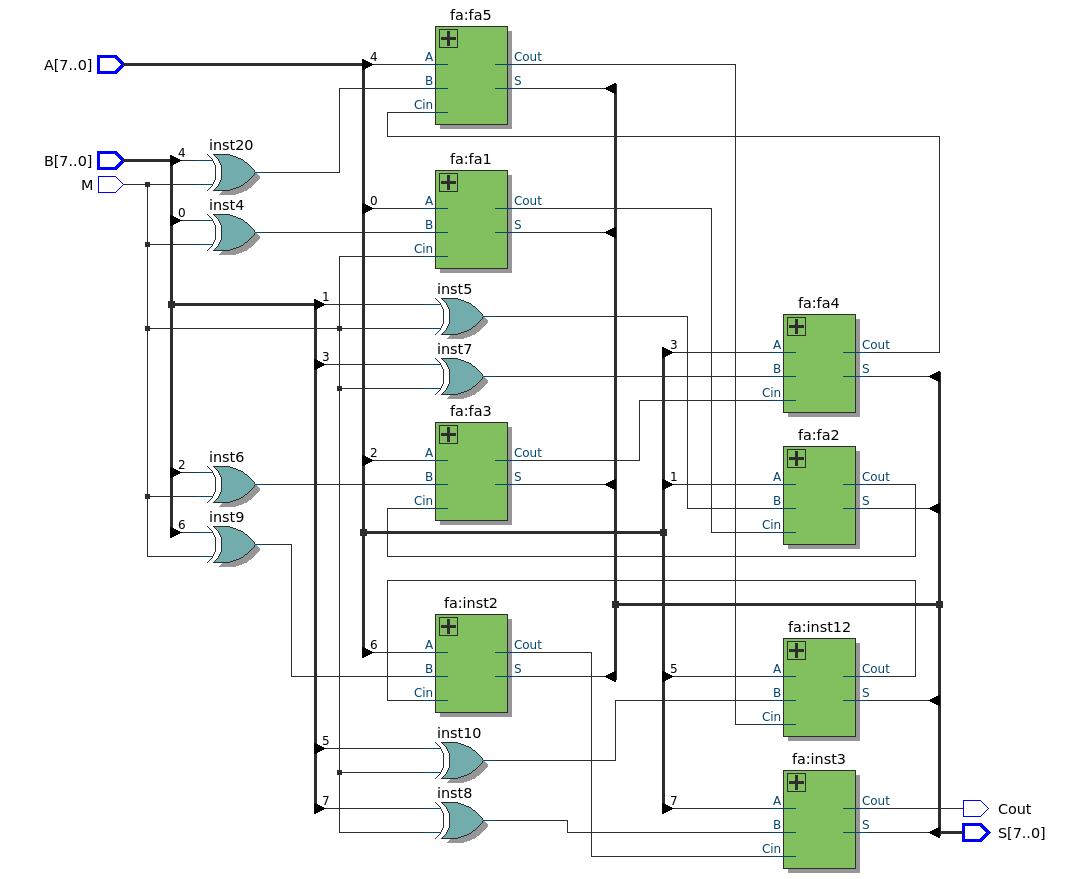
\includegraphics[width=\textwidth]{images/netlist.jpg}
    \caption{Captura de tela do netlist}
\end{figure}

\begin{figure}[H]
    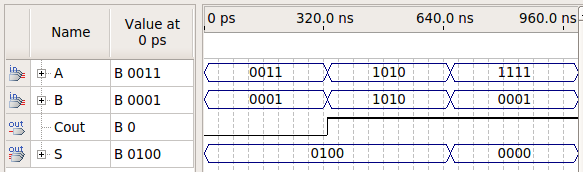
\includegraphics[width=\textwidth]{waveform.png}
    \caption{Captura de tela da simulação em forma de onda com atraso}
\end{figure}

\section{Arquivo de restrições}

\begin{lstlisting}[caption=constraints.sdc]
create_clock -name clk -period 20 [get_ports CLK]

set_input_delay -clock clk -max 0.2 [all_inputs]
set_input_delay -clock clk -min 0.01 [all_inputs]
set_output_delay -clock clk -max 0.2 [all_outputs]
set_output_delay -clock clk -min 0.01 [all_outputs]  
\end{lstlisting}

\end{document}
